% Options for packages loaded elsewhere
\PassOptionsToPackage{unicode}{hyperref}
\PassOptionsToPackage{hyphens}{url}
%
\documentclass[
]{article}
\usepackage{amsmath,amssymb}
\usepackage{iftex}
\ifPDFTeX
  \usepackage[T1]{fontenc}
  \usepackage[utf8]{inputenc}
  \usepackage{textcomp} % provide euro and other symbols
\else % if luatex or xetex
  \usepackage{unicode-math} % this also loads fontspec
  \defaultfontfeatures{Scale=MatchLowercase}
  \defaultfontfeatures[\rmfamily]{Ligatures=TeX,Scale=1}
\fi
\usepackage{lmodern}
\ifPDFTeX\else
  % xetex/luatex font selection
\fi
% Use upquote if available, for straight quotes in verbatim environments
\IfFileExists{upquote.sty}{\usepackage{upquote}}{}
\IfFileExists{microtype.sty}{% use microtype if available
  \usepackage[]{microtype}
  \UseMicrotypeSet[protrusion]{basicmath} % disable protrusion for tt fonts
}{}
\makeatletter
\@ifundefined{KOMAClassName}{% if non-KOMA class
  \IfFileExists{parskip.sty}{%
    \usepackage{parskip}
  }{% else
    \setlength{\parindent}{0pt}
    \setlength{\parskip}{6pt plus 2pt minus 1pt}}
}{% if KOMA class
  \KOMAoptions{parskip=half}}
\makeatother
\usepackage{xcolor}
\usepackage[margin=1in]{geometry}
\usepackage{graphicx}
\makeatletter
\newsavebox\pandoc@box
\newcommand*\pandocbounded[1]{% scales image to fit in text height/width
  \sbox\pandoc@box{#1}%
  \Gscale@div\@tempa{\textheight}{\dimexpr\ht\pandoc@box+\dp\pandoc@box\relax}%
  \Gscale@div\@tempb{\linewidth}{\wd\pandoc@box}%
  \ifdim\@tempb\p@<\@tempa\p@\let\@tempa\@tempb\fi% select the smaller of both
  \ifdim\@tempa\p@<\p@\scalebox{\@tempa}{\usebox\pandoc@box}%
  \else\usebox{\pandoc@box}%
  \fi%
}
% Set default figure placement to htbp
\def\fps@figure{htbp}
\makeatother
\setlength{\emergencystretch}{3em} % prevent overfull lines
\providecommand{\tightlist}{%
  \setlength{\itemsep}{0pt}\setlength{\parskip}{0pt}}
\setcounter{secnumdepth}{-\maxdimen} % remove section numbering
\usepackage{graphicx}
\usepackage{float}
\usepackage{booktabs}
\usepackage{array}
\usepackage{xcolor}
\usepackage{bookmark}
\IfFileExists{xurl.sty}{\usepackage{xurl}}{} % add URL line breaks if available
\urlstyle{same}
\hypersetup{
  hidelinks,
  pdfcreator={LaTeX via pandoc}}

\author{}
\date{\vspace{-2.5em}}

\begin{document}

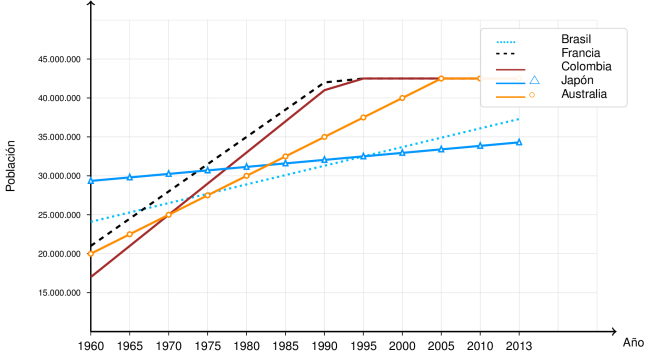
\includegraphics[width=14cm,height=\textheight,keepaspectratio]{grafica_poblaciones_paises.png}

\section{Question}\label{question}

La gráfica muestra información de las poblaciones de 5 países desde 1960
hasta 2013.

Los datos representan la evolución demográfica de diferentes naciones a
lo largo de más de cinco décadas, mostrando distintas tendencias de
crecimiento poblacional.

Aproximadamente, ¿en qué año las poblaciones del País 2 y del País 5
fueron iguales?

\subsection{Answerlist}\label{answerlist}

\begin{itemize}
\tightlist
\item
  \begin{enumerate}
  \def\labelenumi{\arabic{enumi}.}
  \setcounter{enumi}{1988}
  \tightlist
  \item
  \end{enumerate}
\item
  \begin{enumerate}
  \def\labelenumi{\arabic{enumi}.}
  \setcounter{enumi}{1959}
  \tightlist
  \item
  \end{enumerate}
\item
  \begin{enumerate}
  \def\labelenumi{\arabic{enumi}.}
  \setcounter{enumi}{1989}
  \tightlist
  \item
  \end{enumerate}
\item
  \begin{enumerate}
  \def\labelenumi{\arabic{enumi}.}
  \setcounter{enumi}{1994}
  \tightlist
  \item
  \end{enumerate}
\end{itemize}

\section{Solution}\label{solution}

Para resolver este problema, debemos identificar el punto donde las
líneas del País 2 (línea discontinua negra) y del País 5 (línea continua
naranja con círculos) se intersectan en la gráfica.

\textbf{Análisis visual de las tendencias:}

\begin{itemize}
\tightlist
\item
  \textbf{País 2}: Inicia con una población menor pero presenta un
  crecimiento más acelerado
\item
  \textbf{País 5}: Comienza con una población mayor pero su crecimiento
  es más moderado
\end{itemize}

\textbf{Identificación del punto de intersección:}

Observando cuidadosamente la gráfica, podemos ver que las dos líneas se
cruzan aproximadamente en el año \textbf{1989}, donde ambas poblaciones
alcanzan un valor similar de aproximadamente 35-37 millones de
habitantes.

\textbf{Verificación:} - Antes de 1989: País 5 \textgreater{} País 2 -
Después de 1989: País 2 \textgreater{} País 5

\subsection{Answerlist}\label{answerlist-1}

\begin{itemize}
\tightlist
\item
  \textbf{Verdadero}. El año 1989 corresponde al punto de intersección
  visual entre las líneas del País 2 y País 5.
\item
  \textbf{Falso}. 1960 - inicio del período analizado.
\item
  \textbf{Falso}. 1990 - década de referencia común.
\item
  \textbf{Falso}. 1995 - confusión con otro cruce.
\end{itemize}

\section{Meta-information}\label{meta-information}

exname: Intersección Poblaciones Países Gráfica Líneas extype: schoice
exsolution: 1000 exshuffle: TRUE exsection: Estadística/Interpretación
de Gráficas

\end{document}
